%!TEX program = xelatex
% 导言区
\documentclass[12pt, letterpaper]{article}
% 文档区
\usepackage{caption}	% 可以设置脚注的各种性质
\usepackage{graphicx}	% 使用图片
\usepackage{subfigure}	% 使用子图
\usepackage{wrapfig}	% 使用嵌入的图片
\usepackage{color}	% 字体颜色
\usepackage{xcolor}
\usepackage{fullpage}	% 顾名思义
\usepackage{ctex}	% 中文支持
\usepackage{ulem}	% 字体删除线
\usepackage{amsmath}	% 公式换行
\usepackage[colorlinks,linkcolor=blue]{hyperref}	% 插入超链接
\usepackage{mathrsfs}  	% 花体


\title{判别函数}

% 正文区
\begin{document}
% 标题
\maketitle
% 目录
\tableofcontents
\newpage
贝叶斯决策是决策论中的一种。决策论,是对输入进行分类判决。
\textbf{分类器是多种多样的,贝叶斯判别只是其中一种}。有非常多的方法来表述模式分类器,其中用的最多的是一种判别函数$g_i(\mathbf{x})$的形式,如果对于所有的$j\neq i$,有
\begin{equation}
g_i(\mathbf{x})>g_j(\mathbf{x})
\end{equation}
则分类器就会把这个特征向量$\mathbf{x}$判断为$w(i)$。本章就是要研究这个小小的判决函数。
\section{线性判别函数}
这种模型无需估计数据集的分布情况,它只关心概率$P(y|\mathbf{x})$,称为判别模型。
而贝叶斯网络关心数据集中$x,y$的联合概率分布$P(\mathbf{x},y)$,因此称为生成模型。实际应用中的生成模型经常会根据贝叶斯公式转化为$P(\mathbf{x}|y)P(y)$
线性判决函数是指由$\mathbf{x}$的各个分量的线性组合而成的函数:
\begin{equation}
g(\mathbf{x})=\mathbf{w}^T\mathbf{x}+w_0
\end{equation}
其中,$\mathbf{w}=(w_1,w_2,\ldots,w_n)^T$称为权向量,$\mathbf{x}=(x_1,x_2,\ldots,x_n)^T$。$g_i(\mathbf{x})$也可以进一步表示为:
\begin{equation}
g_i(\mathbf{x})=\mathbf{w'}^{T}\mathbf{x'}
\end{equation}
其中,$\mathbf{w'}=(w_0,w_1,\ldots,w_n)^T$,称为增广权向量;$\mathbf{x'}=(1,x_1,x_2,\ldots,w_n)^T$,称为增广模式向量。下面的文字不采用这种形式。
\subsection{相关参数定义}
\begin{itemize}
\item 输入样本$\mathbf{x}$:是一个$d$维向量(有$d$个特征值)(公式中表现为$n$),有$N$个样本数量。可以被表示成一个$d\times N$的矩阵。
\item 权阈值、偏置:$w_0$:一般我们会把$0$作为判决函数的分界。用多少都无所谓,因为可以通过$w_0$调节到$0$,当使用$0$时,$w_0$显然是一个阈值,决定着类别的归属。
\item 权向量:$\mathbf{w}$,和$\mathbf{x}$维度相同的系数(参数)矩阵。判别函数的形式加入确定为线性判别函数,那么剩下的就是求该系数矩阵。
\item 特征空间:拥有$d$维度特征的所有向量的集合。
\item $[x_1,x_2,x_3]$和$[x_1\ x_2\ x_3]$是一样的,都是行向量。$[x_1; x_2; x_3]$是列向量,把分号换成换行也是列向量。
\end{itemize}
\subsection{两类情况}
两类分类器的判决规则一般是这样的:$g(\mathbf{x})>0$则判断为$w_1$,如果$g(\mathbf{x})<0$则判断为$w_2$。
显然$g(\mathbf{x})=0$的解$\mathbf{x}$定义了一个判定面。当$g(\mathbf{x})$是线性的,这个平面被称为“超平面”。假设$x_1$、$x_2$是判定面上的两个点,那么就有:
$$\mathbf{w}^T\mathbf{x}_1+w_0=\mathbf{w}^T\mathbf{x}_2+w_0$$
稍微变动一下就可以得到:
\begin{equation}
\mathbf{w}^T(\mathbf{x}_1-\mathbf{x}_2)=0
\end{equation}
这意味着,$\mathbf{w}$和判定面上的任意向量都垂直,\textbf{即}$\mathbf{w}$\textbf{是判定面的法向量}。

对于特征空间中的任意一点,有:
\begin{equation}
\mathbf{x}=\mathbf{x}_p+r\frac{\mathbf{w}}{||\mathbf{w}||}
\end{equation}
以上公式可以这么理解:$\mathbf{x}_p$是$\mathbf{x}$在判定面$\mathbf{H}$的投影向量,$r$是该点到超平面的算术距离(有正负,代表不同的平面)。$\frac{\mathbf{w}}{||\mathbf{w}||}$是发向量的单位向量。且显然$g(\mathbf{x}_p)=0$,那么就会有:
$$g(\mathbf{x})=\mathbf{w}^T\mathbf{x}+w_0=r||\mathbf{w}||$$。假如$w_0=0$,说明方程具有其次形式,超平面$\mathbf{H}$通过远点。$w_0>0$说明原点在正侧,反之原点在负侧。

简言之:\textbf{超平面$\mathbf{H}$的方向由法向量$\mathbf{w}$确定方向,由阈值权$\mathbf{w_0}$确定位置。判别函数$g(\mathbf{x})$正比于$\mathbf{x}$到超平面的代数距离(带正负号)}。

\subsection{多类情况}
以上的两类情况都是线性判别函数,但是分类器也完全可以是完全分线性的。
例如下面三种思路中,前两种都是线性的思路,而第三种的分界并不是一个线性。
多类的情况可以化为多种两类的情况,有以下三种转化思路:
\begin{enumerate}
\item 把$c$类问题转化为$c$个两类问题。

\qquad 即对于每一类,我只管这一类,其他的所有类被划分成了同一类。这种转化方法,需要$c$个判别函数。只需要$c$个判别函数,相较于类别$2$是一个优点。
\item 使用$\frac{c(c-1)}{2}$个函数(由组合数$C_n^2$得到),每一个线性判别函数只对其中两个类别进行分类。

\qquad 需要的判别函数较多,是一个缺点。
由于一种模式的分布要比M-1种模式的分布更为聚集,因此多类情况2对模式是线性可分的可能性比多类情况1更大一些(这是多类情况2的一个优点)。


\item 通过定义c个判别函数,根据$(1)$的定义进行计算。在线性判别中,无法划分$c$个函数的,因为线性判决时比较在直线的那一侧,是两两成对的。

\qquad 方法$1$和方法$2$都可能湖出现模糊区域,无法判别。该方法构造的分类器又被称为“线性机”,线性机把特征空间氛围$c$个判决区域$R_i$。

\qquad 显然,当$\mathbf{x}$处于区域$i$时,其判决函数$g_i(\mathbf{x})$最大。
后文将会看到,这种判别方式的参数$\mathbf{w}$的求法称为多类模式下的\textbf{感知器算法}。

\end{enumerate}
\section{广义线性判别函数}
广义线性判别函数的出发点:
\begin{itemize}
\item 线性判别函数简单,容易实现;
\item 非线性判别函数复杂,不容易实现;
\item 若能将非线性判别函数转换为线性判别函数,则有利于模式分类的实现。
\end{itemize}
\subsection{基本思想——非线性映射}
把本来\textbf{线性不可分}的样本集$\{\mathbf{x}\}$经过一次非线性变换,变成一个线性可分的样本集$\{\mathbf{x}^*\}$
先不用管怎么找得到,但是\textbf{总能找到一种变换,达到上述目的}。变化之后的样本的维度要大于原样本集的样本维度。
这种非线性转换的过程可以形式化为:
\begin{equation}
\mathbf{x^*}=(f_1(\mathbf{x}),f_2(\mathbf{x}),\ldots,f_k(\mathbf{x})),\qquad k>n
\end{equation}
即$\mathbf{x^*}$各个分量是$\mathbf{x}$的单值函数。
\begin{equation}
But\ why\ k\ is\ greater\ than\ n\ ?
\end{equation}
将会在后面证明。
\subsection{关于映射函数\texorpdfstring{$f_i(\mathbf{\mathbf{\mathbf{x}}})$}{}的讨论}
\begin{enumerate}
\item \textbf{$f_i(\mathbf{x})$是线性函数}

\qquad 例如$f_i(\mathbf{x})=x_i$(取$\mathbf{x}$中的第$i$个)。此时$\mathbf{x^*}=\mathbf{x}$。此时的广义线性判决时仍然是原线性判决式:$g(\mathbf{x})=\mathbf{w}^T\mathbf{x}+w_0$。

\item \textbf{当$f_i(\mathbf{x})$是二次多项式函数}

\qquad(这意味着广义线性判决函数也是一个二次的多项式函数)

\begin{enumerate}
\item 当$\mathbf{x}$是二维的,即$\mathbf{x}=(x_1, x_2)^T$

\qquad 此时判别函数可以表示为:
\begin{equation}
d(\mathbf{x})=w_{11}x_1^2+w_{22}x_2^2+w_{12}x_1x_2+w_1x_1+w_2x_2+w_3
\end{equation}
显然此时有:
$$\mathbf{x^*}=(x_1^2,x_1x_2, x_2^2,x_1,x_2,1)^T$$
远大于$\mathbf{x}$的维度。
$$\mathbf{w}=(w_{11},w_{12},w_{22},w_1,w_2,w_3)^T$$
\item 当$\mathbf{x}$是$n$维的。

(有几维向量就可以构造最多几阶的判别函数,此处限制为两阶了而已。)

\qquad 此时的判决函数为:
\begin{equation}
d(\mathbf{x})=\sum_{j=1}^nw_{jj}x_j^2+\sum_{j=1}^{n-1}\sum_{k=j+1}^{n}w_{jk}x_jx_k+\sum_{j=1}^nx_j+w_{n+1}
\end{equation}
显然此时有:
\begin{equation}
f_i(\mathbf{x})=x_{p_{1}}^sx_{p_2}^t,\qquad p_1,p_2=1,2,3\ldots,n,\qquad t=0,1
\end{equation}
对应的有:
\begin{equation}
w_i=w_{p_1^sp_2^t},\qquad p_1,p_2=1,2,3\ldots,n,\qquad t=0,1
\end{equation}
显然此时有$n + \frac{n(n-1)}{2} + n + 1 = \frac{(n+1)(n+2)}{2} $个维,大于原样本集$\{x\}$的$n$维样本集。而这仅仅是讨论了二次的转化函数,当$f_i(\mathbf{x})$推广到$n$维(样本有$n$维的话,最多可以构造出$n$阶的判别函数,也就有$n$阶的转化函数$f_i(\mathbf{x})$),\underline{此时$\{x^*\}$的维度将会远远大于$n$维。}

注意参数$w$的所有数值都是未知的。非线性变化的形式已经确定下来后,$w$就变成了唯一的参数,这也是第$5$节开始讨论的。
\end{enumerate}
\item \textbf{继续推广:$f_i(\mathbf{x})$推广到$n$维}

本有$n$维的话,最多可以构造出$n$阶的判别函数,也就有$n$阶的转化函数$f_i(\mathbf{x})$。
显而易见,把$(9)$式推广搭配$n$维空间可以得到:
\begin{equation}
f_i(\mathbf{x})=x_{p_1}^{s_1}x_{p_2}^{s_2}\ldots x_{p_r}^{s_r},\qquad p_1,p_2,\ldots,p_r=1,2,\ldots,n,\qquad s_1,s_2,\ldots,s_r=0,1
\end{equation}
其判别函数$d(\mathbf{x})$的$r$次项的表达式也是显而易见的(虽然写起来很麻烦):
\begin{equation}
d^{(r)}(\mathbf{x})=\sum_{p_1=1}^n\sum_{p_2=p_1}^n\sum_{p_3=p_2}^n\ldots\sum_{p_r=p_{r-1}}^nw_{p_1p_2\ldots p_r}x_{p_1}x_{p_2}\ldots x_{p_r}+d^{(r-1)}(x)
\end{equation}
对于$n$维的$\mathbf{x}$向量,使用$r$次多项式,$d(\mathbf{x})$系数的总项数,即转化后的维数为:
\begin{equation}
N_w=C_{n+r}^r=\frac{(n+r)!}{r!n!}
\end{equation}
例如:$r=2$时,即$2.(b)$所讨论的内容,$N_w=\frac{(n+2)!}{2!n!}=\frac{(n+2)(n+1)}{2}$。
$r$是最高次项,$n$是维度。
\end{enumerate}
\subsection{结论}
\subsubsection*{$d(\mathbf{x}$)的项数随$r$和$n$的增加会迅速增大}
即使原来模式$\mathbf{x}$的维数不高,若采用次数$r$较高的多项式来变换,也会使变换后的模式$\mathbf{x^*}$的维数很高,给分类带来很大困难。
\subsubsection*{实际情况可只取r=2,或只选多项式的一部分}
例如$r=2$时只取二次项,略去一次项(因为相比于高次项,低次项的影响小一个数量级),以减少$\mathbf{x^*}$的维数。

只能得到二次的判决函数,相当于能计算得到二阶的判别函数。
\section{分段线性判别函数}

\subsection{出发点}

\begin{wrapfigure}{l}{6.5cm}
\centering
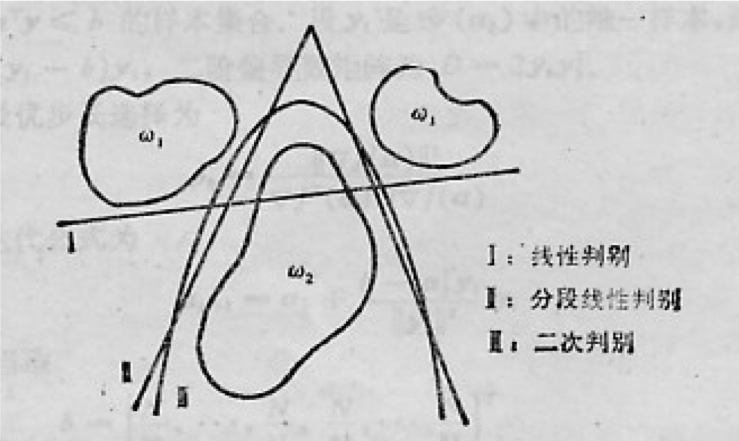
\includegraphics[scale=0.5]{三种判决函数.png}
\captionsetup{font={footnotesize}}   
\caption{三种不同的判决函数}
\end{wrapfigure}

线性判别函数在进行分类决策时是最简单有效的,但在实际应用中,常常会出现不能用线性判别函数直接进行分类的情况。

尽管可以使用广义线性判别的方法,但是随着维度的增加和判决函数的阶次的增加,使得解析和计算在高纬空间上遇到困难。

要注意的是,我们一般只能采用$r=2$次项,即在原特征空间$\mathscr{R}^d$中,使用一个二次函数去划分样本集${\mathbf{x}}$。


\subsection{主要思想:逼近}
分段线性的主要思想是,\textbf{使用一个分段线性判别函数来逼近}这个二次曲线(或更高次曲线)。

\subsection{设计一个分段线性判别函数}
\begin{figure}[h]
	\centering 

	\captionsetup{font={footnotesize}}  

	\subfigure[两类最小距离分类法]
	{ 
	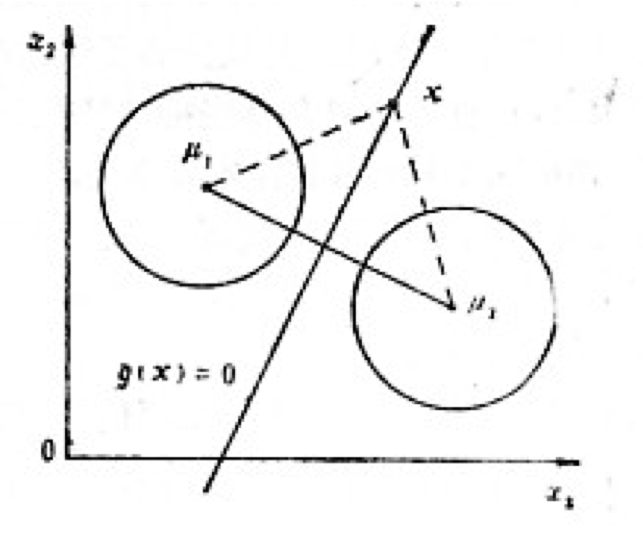
\includegraphics[scale=0.55]{最小距离分类.png}
	}
	\hspace*{0.5in}
	\subfigure[多类的最小距离法]
	{ 
	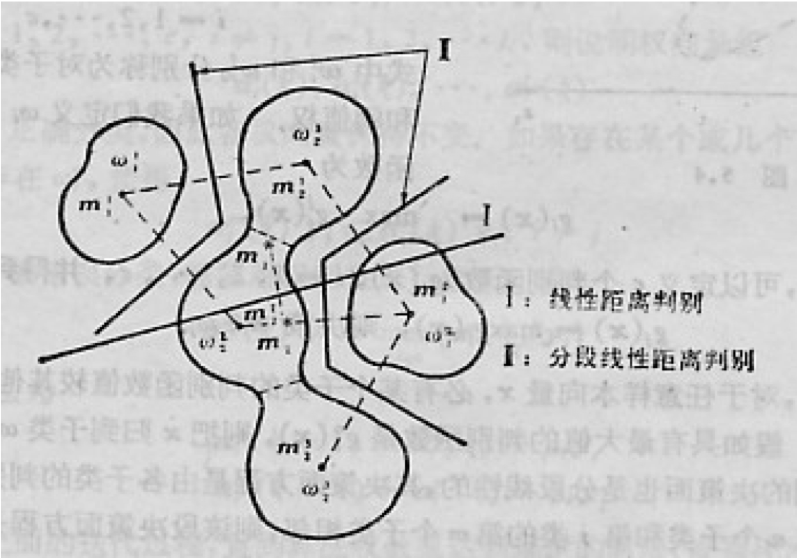
\includegraphics[scale=0.5]{多类的最小距离法.png}
	}
	\caption{最小距离分类}
	\label{fig:subfig} 
\end{figure}

分段线性的判别函数,\textbf{它比线性的效果好,又比非线性的简单。}
\textbf{如何分段}是最核心的问题,\textbf{最小距离分类法}是最常用的办法。它计算两个类别的中心,并以两个中心之间线段的的垂直平分线作为分段的一部分。

在多个类别时,计算多个垂直平分线并想办法把他们联结起来,如图所示。


\section{降维——Fisher分析法}
\subsection{降维}
广义线性判别函数通过增加维度来进行非线性变换,从而实现线性可分。通过降维也可以实现相似的效果,Fisher算法就是一个降维算法(降到一维)。
\subsubsection*{出发点:}
\begin{itemize}
\item 应用统计方法解决模式识别问题时,一再碰到的问题之一就是维数问题。
\item 在低维空间里解析上或计算上行得通的方法,在高维空间里往往行不通。
\item 因此,\textbf{降低维数有时就会成为处理实际问题的关键。}
\end{itemize}

\subsection{问题描述}
\subsection{从\texorpdfstring{$\mathscr{R}^d$}{}空间到
\texorpdfstring{$\mathscr{R}^1$}{}空间的一般数学变换方法
}
\subsection{Fisher准则函数的定义}
\subsection{基于最佳变换向量\texorpdfstring{$\mathbf{w^*}$}{}的投影}
\underline{以上知识确定了算法的形式}:
\begin{itemize}
\item 是否是线性分类器
\item 分几类
\item 有无升(广义线性)/降维(Fisher)操作
\end{itemize}
下面需要确定具体的参数,感知器算法就是用来确定系数的。

\section{确定判别函数参数——感知器算法}
无论是升维还是降维,都是对数据进行处理并\textbf{确定好判别函数的形式}。
\subsection{算法思想}
\subsubsection*{出发点}
\begin{itemize}
\item 只要判别函数的形式一确定,\textbf{无论是线性的还是非线性的},剩下的问题就是确定它的系数。
\item \textbf{通过对已知样本的训练和学习来得到系数}是机器学习的一大主要方法。
\item 感知器算法,就是上述算法之一。训练样本模式的迭代和学习,产生\textbf{线性(或广义线性)可分的模式判别函数}。
\end{itemize}

\subsubsection*{背景$^*$}
“感知器”一词出自于20世纪50年代中期到60年代中期人们对一种分类学习机模型的称呼,它是属于有关动物和机器学习的仿生学领域中的问题。
当时的一些研究者认为感知器是一种学习机的强有力模型,后来发现估计过高了,但发展感知器的一些相关概念仍然沿用下来。


\subsubsection*{基本思想}
采用感知器算法(Perception Approach)能通过对训练模式样本集的“学习”得到判别函数的系数。

\subsubsection*{确定性方法}
确定性方法是一类用于确定参数的方法的总称,该类方法不需要知道样本中各模式的统计性质(不需要对统计性质作出假设)。因此被称为“确定性算法”。

\subsection{感知器的二分类训练算法}
\subsubsection*{文字描述}
感知器算法实质上是一种赏罚过程:
\begin{itemize}
\item 对正确分类的模式则“赏”,实际上是“不罚”,即权向量不变。
\item 对错误分类的模式则“罚”,使$\mathbf{w}(k)$加上一个正比于$\mathbf{x_k}$的分量。
\item 当用全部模式样本训练过一轮以后,\textbf{只要有一个模式是判别错误的,则需要进行下一轮迭代,即用全部模式样本再训练一次}。
\item 如此不断反复直到全部模式样本进行训练都能得到正确的分类结果为止。
\end{itemize}
只要模式类别是线性可分的,就可以在有限的迭代步数里求出权向量。(证明见Appendix)

\subsubsection*{数学描述}
对于一个线性判别函数$g(x)=\mathbf{w}^T\mathbf{x}$,$\mathbf{w}$是增广权向量,$\mathbf{x}$是增广模式向量。
对于属于类别$w_1$的样本$\mathbf{x}$,有$g(\mathbf{x})>0$;对于属于类别$w_2$的样本$\mathbf{x}$,有$g(\mathbf{x})\leq0$。
\subsubsection*{讨论判决正误与否以及对应的惩罚函数}
\begin{enumerate}
\item 当$\mathbf{x}$属于$w_1$,且$g(\mathbf{x})>0$时候,作出了正确判断。因此权向量不变,即:$w(k+1) = w (k)$。
\item 当$\mathbf{x}$属于$w_1$,但是$g(\mathbf{x})\leq0$时候,即作出了错误判断。因此权向量要收到“惩罚”(进行矫正),即:$w(k+1) = w (k)+C\mathbf{x_k}$。
\item 当$\mathbf{x}$属于$w_2$,且$g(\mathbf{x})\leq0$时候,作出了正确判断。因此权向量不变,即:$w(k+1) = w (k)$。
\item 当$\mathbf{x}$属于$w_2$,但是$g(\mathbf{x})>0$时候,即作出了正确判断。因此权向量需要矫正,矫正方向应该和情况$2$相反,即:$w(k+1) = w (k)-C\mathbf{x_k}$。
\end{enumerate}

为了统一公式,可以把所有属于$w_2$的样本都$\times-1$,可以使得公式可以统一为:
\begin{equation}
\mathbf{w}(k+1)=\left\{
\begin{aligned}	
& \mathbf{w}(k) \qquad &\mathbf{w}\mathbf{x}>0\\
& \mathbf{w}(k)+C\mathbf{x_k} &\qquad \mathbf{wx}\leq0
\end{aligned}
\right.
\end{equation}

\section{感知器算法的多模式分类}
多模式分类下的感知器算法其实是线性分类中的第三种多类情况(1.3.3)下的系数$\mathbf{w}$。

多类模式下依旧是使用迭代的思想。

假如有$M$中模式,计算出每一个类别的判决函数
$g_i(\mathbf{x})$,对于$M$类会有$M$个判决函数。

\textbf{判罚依据:对于属于第$i$类的样本数据$\mathbf{x}$,在正确分类的情况下,$g_i(\mathbf{x})$是$M$个判决函数中最大的那一个。}



\subsection{迭代过程}

\subsubsection*{文字描述}
在第$k$次迭代,输入一个属于$i$类的样本数据$\mathbf{x}$,计算$M$个判决函数。根据判罚依据,假如判决正确。$\mathbf{w}$不变,即$\mathbf{w(k+1)=w(k)}$。当\textbf{第一次发现}存在一个类别$j$,使得判决错误,即:$g_i(k)\leq g_j(k)$。那么就要$i$和$j$类都进行“矫正”:
\begin{equation}
\begin{aligned}
\mathbf{w_i}(k+1)=\mathbf{w_i}(k)+C\mathbf{x}\\
\mathbf{w_j}(k+1)=\mathbf{w_j}(k)-C\mathbf{x}\\
\end{aligned}
\end{equation}
对于其他的判别函数,有:
$$\mathbf{w_l}(k+1)=\mathbf{w_l}(k),\qquad l=1,2,3,\ldots,M,l\neq i,l\neq j$$
然后输入下一个样本$\mathbf{x'}$。其中$C$是一个正常数。
迭代完一轮之后,再迭代下一轮,直到所有的$\mathbf{w}$都不发生变化,即所有的样本都分类成功。

\subsection{使用迭代计算参数的确定性分类器的一些讨论}
\subsubsection*{训练样本和测试样本}
这里的分类算法都是通过\textbf{模式样本(训练数据)}来确定判别函数的系数,但一个分类器的判断性能最终要受并\textbf{未用于训练的(测试数据)}那些未知样本来检验。
\subsubsection*{感知器算法对数据的要求}
要使一个分类器设计完善,必须采用有代表性的训练数据,它能够合理反映模式数据的整体。
\subsubsection*{要获得一个判别性能好的\textbf{线性分类器},究竟需要多少训练样本?
}
\begin{itemize}
\item 直观上是越多越好,但实际上能收集到的样本数目会受到客观条件的限制;

\item 过多的训练样本在训练阶段会使计算机需要较长的运算时间;


\item \textbf{一般来说,合适的样本数目可如下估计:
	若k是模式的维数,令C=2(k+1),则通常选用的训练样本数目约为C的10~20倍。
}
\end{itemize}



\section{推广:可训练的确定性分类器的迭代过程}
对于感知器算法,其\textbf{更新策略}可以写为如$(15)$所示:
$$
\mathbf{w}=\left\{
\begin{aligned}
& \mathbf{w}(k) \\
& \mathbf{w}(k)+C\mathbf{x_k}
\end{aligned}
\right.
$$
感知器算法可以把梯度堪称是$C^{`}\mathbf{x_k}$的一个特例。下面将会把$C\mathbf{x_k}$替换为一般形式的$\mathbf{J}(\mathbf{w}, \mathbf{x})$。


\subsection{梯度法}
\subsubsection*{梯度的定义}
假如有$g(\mathbf{x})$,且$\mathbf{x}=(x_1,x_2,\ldots,x_n)^T$维度的向量。根据高等数学中的高纬度情况下的求导公式为:
$$
\nabla g(\mathbf{x})=\frac{d}{d\mathbf{x}}g(\mathbf{x})=(\frac{\partial g}{\partial x_1},\frac{\partial g}{\partial x_2},\ldots,\frac{\partial g}{\partial x_n})^T
$$

\subsubsection*{再次理解感知器算法}
对于二类分类器,当第$k$次迭代的时候,此时的$\mathbf{w}=\mathbf{w_k}$,此时的输入是$\mathbf{x}$,假设有:
$$
\mathbf{J}(\mathbf{w},\mathbf{x})=
\left\{
\begin{aligned}
&\mathbf{w_k}\mathbf{x}\qquad &\mathbf{w_k}x>0,\\
&0 \qquad &\mathbf{w_k}x\leq 0
\end{aligned}
\right .
$$

则此时的迭代公式为:

\begin{equation}
\begin{aligned}
\mathbf{w}(k+1)&=\mathbf{w}(k)+C\left\{ \frac{\partial J(\mathbf{w}, \mathbf{x})}{\partial \mathbf{w}}\right\}_{\mathbf{w}=\mathbf{w_K}}\\
&=
\left\{
\begin{aligned}
& \mathbf{w}(k) \qquad &\mathbf{w}\mathbf{x}>0\\
& \mathbf{w}(k)+C\mathbf{x_k} &\qquad \mathbf{wx}\leq0
\end{aligned}
\right.
\end{aligned}
\end{equation}
C是一个正比例步长因子。注意这里的$\mathbf{x}$和\textbf{定义}里的$\mathbf{x}$不是一个。同(15)。

形象地说,梯度法的过程是先任选一个初始权向量$w(1)$,计算准则函数$J$的梯度,然后从$w(1)$出发,在最陡方向(梯度方向)上移动某一距离得到下一个权向量$w(2)$

\subsubsection*{梯度法的定义} 
若正确地选择了准则函数$J(w,x)$,则当权向量$w$是一个解时,$J$达到极小值($J$的梯度为零)。由于权向量是按$J$的梯度值减小,因此这种方法称为梯度法(最速下降法)。

\subsubsection*{梯度因子\textbf{C}}
为了使权向量能较快地收敛于一个使函数J极小的解,C值的选择是很重要的。
\begin{itemize}
\item 
若C值太小,则收敛太慢;
\item 
若C值太大,则搜索可能过头,引起发散。
\end{itemize}

\subsection{梯度法最简单的训练方式:固定增量的逐次调整算法}
固定增量的主次调整法其实就是上面讨论的内容。
其中$\mathbf{J}(\mathbf{w},\mathbf{x})$可以统一写为:
\begin{equation}
\mathbf{J}(\mathbf{w},\mathbf{w})=\frac{|\mathbf{w}^T\mathbf{x}|-\mathbf{w}^T\mathbf{x}}{2}
\end{equation}
初始权向量w(1)的值可任选。
% 感知器算法是这类算法的一个特例
\subsection{最小平方误差(LMSE)算法}
\subsubsection{感知器的缺点以及LMSE的特点}
LMSE算法的出发点是为了克服感知器算法的缺点:
感知器算法只有不同的类别在特征空间中线性可分的时候,才会\textbf{收敛}。

其次,需要迭代的次数无法事前算出。

因此可能会出现这种情况:\textbf{随着训练的进行,样本一个一个、一轮一轮的迭代,但是结果始终不见收敛。}

而且更糟糕的是,我们\textbf{无法知道是由于训练集线性不可分造成的,还是由于迭代次数不足造成的。}

\textbf{最小平方误差(LMSE)算法,除了对可分模式是收敛的以外,对于类别不可分的情况也能指出来。}实际上,LMSE是使用数学方法,对于两类情况,指出线性可分的测试特征(当然它的运算更加麻烦,这是它的缺点)。

\subsubsection{符号和数学概念}
\subsubsection*{线性分类器的不等式方程}
对于一个仅有$w_1$、$w_2$两类的线性分类器来说,应该满足以下分类依据:
$$
\begin{aligned}
\mathbf{w}^T\mathbf{x}>0,\quad \forall \mathbf{x}\in w_1\\
\mathbf{w}^T\mathbf{x}<0,\quad \forall \mathbf{x}\in w_2
\end{aligned}
$$

假如把类别$w_2$的样本都乘$-1$,那么对两种模式,判决函数就可以统一为:
$$
\mathbf{w}^T\mathbf{x}>0
$$
其中:$\mathbf{x}=(x_1,x_2,\ldots,x_n)^T$和$\mathbf{w}=(w_1,w_2,\ldots,w_n)^T$都是列向量。可以把所有的样本拼到一个矩阵里面去,得到:
$$
\mathbf{X}=\left(
\begin{aligned}
&\mathbf{x_1}^T\\
&\vdots \\
&\mathbf{x_i}^T\\
-&\mathbf{x_{i+1}}^T\\
&\vdots \\
-&\mathbf{x_N}^T
\end{aligned}
\right)
$$

$$
\mathbf{w}=(w_1,w_2,\ldots,w_n,w_{n+1})^T
$$
其中$\mathbf{X}$矩阵里面的所有的$\mathbf{x}$都是一个n维向量。
因为$\mathbf{w}^T\mathbf{x}=(\mathbf{w}^T\mathbf{w})^T>0$,所以也会有$\mathbf{w}^T\mathbf{w}>0$
所以可以写为:
\begin{equation}
\mathbf{Xw}>\mathbf{0}
\end{equation}
其中,$\mathbf{0}$是零向量。以上就是线性分类器的不等式方程,其中$\mathbf{x}$是一个$N*(n+1)$阶矩阵,$N$是样本数量,$n$是特征维度。
$w$是一个$n*1$维的列向量。该式意味着$\mathbf{Xw}$的矩阵的各个元素都大于零。

对于多类的情况,可以划分为1.3.1类分别进行上述运算。

\subsubsection*{不等式方程的解的存在性}
假设
\begin{equation}
\mathbf{Xw}=\mathbf{b}
\end{equation}
,只要$\mathbf{b}>0$即可。

由于$X$是一个$N*(n+1)$阶的矩阵,样本数量一般远远大于特征维度。因此$\mathbf{Xw}=\mathbf{b}$一般是一个超定方程。
\subsubsection*{MSE解法初步介绍}
假如$\mathbf{X}$是非奇异的,便可以直接求解:$\mathbf{w}=\mathbf{X}^{-1}\mathbf{b}$。但是对于奇异方程,不可求其逆矩阵(当矩阵可逆,该矩阵一定是一个方阵而且满秩)。

但是我们可以通过定义一个误差向量:
$$ \mathbf{e}=\mathbf{Xw-b}$$
并且寻找最小化平法误差和的准则函数:
\begin{equation}
\mathbf{J}(\mathbf{w})=||\mathbf{e}||^2=||(\mathbf{Xw-b})^2||
\end{equation}
寻找某个权向量$\mathbf{w}$使得上式最小,即可得到接近于一个最好的解决。
通过求梯度、求极值的方法,可以得到:当出现梯度为$0$时,会有:
\begin{equation}
\mathbf{X^TXw=X^Tb}
\end{equation}

\textbf{通常}矩阵$\mathbf{X^TX}$是非奇异的方阵,因此上述方程必定有一个唯一的解:

\begin{equation}
\mathbf{w}=\mathbf{(X^TX)^{-1}X^Tb}
\end{equation}
该解是方程$(20)$的$MSE$解(最小误差平方和解)。(值得注意的是当$\mathbf{X}$是非奇异方针,那么逆伪矩阵就是$\mathbf{X}$的逆矩阵。)
\subsubsection*{Make it clear:讨论\texorpdfstring{$(21)$、$(23)$}{PDFstring}的含义}
最小平方误差和作为一个准则函数,通过梯度法逐渐减小最小平方误差来达到最有效果。因此,该算法下,\textbf{最优的效果是J最小。}但是要注意的是,\textbf{J最小的时候并不一定全部分类正确(即便是线性可分的情况)}

$\mathbf{w}$称为方程$(20)$的$MSE$解,但实际上\textbf{这个点只意味着导数为0,却并不是一定是方程真正的解。}这个极致点作为一个约束条件出现在即将进行的推导中,只有满足这个条件,迭代出来的$\mathbf{b}$和$\mathbf{w}$才是极致点。

这个点不一定是方程$(20)$的节可以如下证明:把$(23)$带入$(20)$可得:
\begin{equation}
\mathbf{Xw}=\mathbf{X(X^TX)^{-1}X^Tb}\neq XX^{-1}(X^T)^{-1}X^Tb=b
\end{equation}
这是因为$X$是不可逆的,因此上述推导在大多数情况下并不成立。


矩阵求梯度怎么算?


显然MSE解是由$\mathbf{b}$确定的,\textbf{不同的$\mathbf{b}$会带来不同的性质,这一点作为扩展将会在$7.5$中详细讨论。}

\subsubsection{LMSE-(H-K)算法}
MSE法依靠最小平方误差函数和极值点约束这两个条件,可以在不管样本是否可分都能找到一个权向量,\textbf{虽然不能保证这个向量一定是分类向量},单一定使$\mathbf{J}$最小。
如果裕量$\mathbf{b}$是任意选择的,\textbf{那么我们最多可以说,我们能够保证$||\mathbf{e}||$极小化。}但是并不能保证这个极小值到达了我们可以到达的最小值。而迭代的过程,就是在不断让极小值变小的过程。在此过程中要满足$\mathbf{b}$始终满足条件$\mathbf{b}>0$,且始终满足$\mathbf{w}$和$\mathbf{b}$的约束条件。
\subsubsection*{---Math Warning!---}





\subsubsection{如何根据LMSE看出是否样本集是否线性可分}


\subsection{关于上述两种方法的讨论}
\begin{enumerate}
\item 
固定增量算法:实现相对简单,可直接引伸到多类模式的分类情况,但未提供模式线性可分的测试特征;
\item 
LMSE算法:相对复杂,需要对XTX求逆(维数高时求逆比较困难),但对两类情况,提供了线性可分的测试特征
\item 
其他:MSE算法有两个问题:
\begin{itemize}
\item $\mathbf{X^TX}$可能是奇异的
\item $\mathbf{X}$可能会非常大
\end{itemize}
\href{https://www.youtube.com/watch?v=sKuHAkkvQqU}{请参考此处Youtube课程,查看其后续引出内容} 

\end{enumerate}

\subsection{扩展:LMS算法介绍以及其和LMSE算法、Fisher算法以及bayes算法的关系\texorpdfstring{$^*$}{PDFstring}}

\section{势函数法 — 一种确定性的非线性分类方法}
\section{决策树简介}


\end{document}